\section{Axial Elements}
\label{sec:axial}

An \emph{axial element} is a linear resistant element whose deformation happens in the direction or its directrix only.
The linear elements used by \emph{InkFEM} are a combination of axial and beam elements (see Section~\ref{sec:beams}).


\subsection{Energy Formulation}

The total energy of an axial element\dots

\subsection{Displacement Field And Interpolation Functions}

Let $\vec{u}(x)$ be the displacements field in the axial finite element of length $L$.
$u_1$ is the displacement of the element's node 1 in the X direction, and $u_2$ the displacement of node 2 in the X direction.
The displacements field can be chosen to vary linearly inside the finite element, so it can be interpolated from the values of $u_1$ and $u_2$ like so:

\begin{equation}
  \vec{u}(x) = N_1 u_1 + N_2 u_2
\end{equation}

where:

\begin{equation}
  \begin{split}
    N_1(x) & = 1 - \frac{x}{L} \\
    N_2(x) & = \frac{x}{L} \\
  \end{split}
\end{equation}


\subsection{Distributed Loads}

We consider distributed axial loads that vary linearly with respect to the X direction:

\begin{equation}
  q_x(x) = a + bx
\end{equation}

The work done by these forces can be obtained by the following integration:

\[
  W_{q_x} = \int_{0}^{L} q_x \vec{u}(x) dx = \int_{0}^{L} (a + bx) \left[ \left( 1 - \frac{x}{L} \right) u_1 + \left( \frac{x}{L} \right) u_2 \right] dx
\]

Which yields a result of:

\[
  W_{q_x} =
  \begin{bmatrix}
    \frac{a L}{2} + \frac{b L^2}{6} & \frac{a L}{2} + \frac{b L^2}{3} \\
  \end{bmatrix}
  \begin{bmatrix}
    u_1 \\
    u_2 \\
  \end{bmatrix}
\]

Therefore, a linear axial load $q_x(x)$ can be distributed over the two nodes in the finite element adding the forces:

\begin{equation}
  \begin{split}
    F_x^1 = \frac{a L}{2} + \frac{b L^2}{6} \\
    F_x^2 = \frac{a L}{2} + \frac{b L^2}{3} \\
  \end{split}
\end{equation}

Figure~\ref{fig:axial_finite_element_load_distribution} depicts this distibution of a linear axial load inside a finite element of length L.

\begin{figure}[h]
  \label{fig:axial_finite_element_load_distribution}
  \centering
  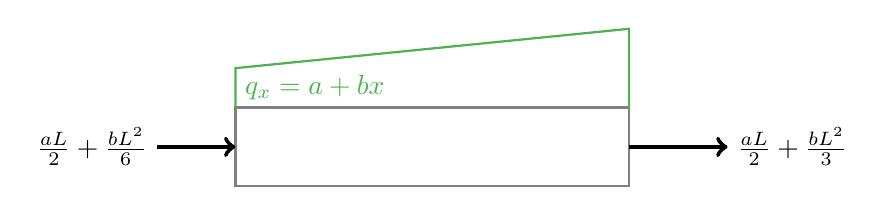
\begin{tikzpicture}
    \draw[gray, thick] (1,0) rectangle (6,1);
    \draw[green!40!gray, thick] (1,1) -- (1,1.5) -- (6,2) -- (6,1);
    \filldraw[green!40!gray] (1,1.25) node[anchor=west] {$q_x = a + bx$};
    \draw[ultra thick, ->] (0,0.5) -- (1, 0.5);
    \draw[ultra thick, ->] (6,0.5) -- (7.25, 0.5);
    \filldraw[black] (0,0.5) node[anchor=east] {$\frac{aL}{2} + \frac{b L^2}{6}$};  
    \filldraw[black] (7.25,0.5) node[anchor=west] {$\frac{aL}{2} + \frac{b L^2}{3}$};  
  \end{tikzpicture}
  \caption{Distribution of a distributed axial load}
\end{figure}


\subsection{Axial Stress}

Once the finite element's node displacements in the X direction $u_1$ and $u_2$ are obtained, the axial stress $\sigma_e$ can be computed as follows:

\[
  \sigma_e = E \epsilon_e = E \left( \frac{u_2 - u_1}{L} \right)
\]

Since we know that inside a bar subject to a distributed axial load $q_x(x)$:

Given the stress inside the element, $\sigma_e$, we can now compute the values of the axial stress in the nodes:

\[
  \begin{split}
    \sigma_e^1 = \sigma_e + \frac{F_x^1}{A} = \sigma_e + \frac{1}{A} \left( \frac{a L}{2} + \frac{b L^2}{6} \right) \\
    \sigma_e^2 = \sigma_e - \frac{F_x^2}{A} = \sigma_e + \frac{1}{A} \left( \frac{a L}{2} + \frac{b L^2}{3} \right) \\
  \end{split}
\]

In the finite element's left node, the axial stress value equals the element's stress plus the left load over the cross section area.
The axial stress at the right node is the element's stress plus the right load over the cross section area.


\subsection{Example}

This example is implemented as an integration test in the \emph{axial\_member\_test.go} to ensure the correct working of the FEM procedure.

Consider an axial member with one of its ends fixed and an axial distributed load that goes from 400 $\frac{\text{N}}{\text{cm}}$ in the fixed end to 0 $\frac{\text{N}}{\text{cm}}$ in the free end.
The bar has a length of 100 cm, a cross section area of 14 $\text{cm}^2$ and is made of a material whose Young modulus is $20 \times 10^6 \frac{\text{N}}{\text{cm}^2}$.
This axial bar is depicted in Figure~\ref{fig:axial_bar_distributed}.

\begin{figure}[h]
  \label{fig:axial_bar_distributed}
  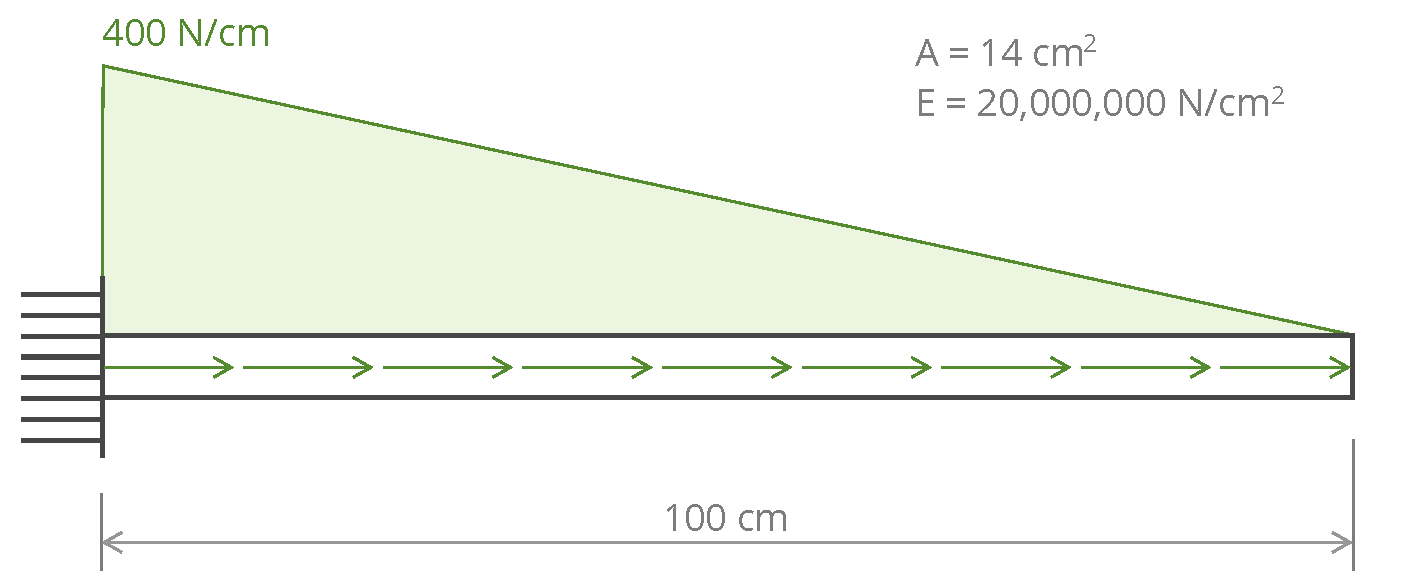
\includegraphics[width=\linewidth]{sections/img/axial_bar_distributed.pdf}
  \caption{Axial bar subject to a distributed load}
\end{figure}

\subsubsection{The Axial Stress}

Let's start by finding the expression in terms of the position x of the axial stress inside the bar.
From mechanics of materials, we know that in an axial member, the normal stress $\sigma$ is:

\[
  \sigma = E \epsilon  
\]
where $E$ is the material's Young modulus and $\epsilon$ is the strain.
Given the displacement field $u(x)$ inside the bar subject to external loads, the strain can be expressed as:

\[
  \epsilon = \frac{du}{dx}  
\]
and therefore:

\[
  \sigma = E \frac{du}{dx}
\]

At the same time, we know that the equilibrium of a differential slice in the bar yields the following relation:

\[
  \frac{\partial \sigma}{\partial x} = - \frac{q_x(x)}{A}  
\]
The distributed load can be formulated as:

\[
  q_x(x) = a + bx = 400 - 4x
\]

We can obtain the analytical value for the stress function of the position x integrating:

\[
  \sigma(x) = - \int \frac{q_x(x)}{A} \,dx 
  = - \int \left( \frac{a + bx}{A} \right) \,dx 
  = \sigma_r - \frac{1}{A} \left( ax + \frac{b x^2}{2} \right)
\]

Where $\sigma_r$ is the normal stress in the fixed end, which can be obtained computing the reaction force first:

\[
  N_r = \frac{400 \frac{\text{N}}{\text{cm}} \times 100 \text{cm}}{2} = 20,000 \text{N}
\]
And then dividing the reaction force $N_r$ by the bar's cross section area A:

\[
  \sigma_r = \frac{20,000 \text{N}}{14 \text{cm}^2} = 1428.57 \frac{\text{N}}{\text{cm}^2}
\]


\subsubsection{The Axial Displacements}

Given the stress-strain equation, to compute the displacement in the x direction:

\[
  du = \frac{\sigma}{E} dx  
\]
Integrating:

\[
  u(x) = \cancel{u_r} + \frac{1}{E} \int \sigma(x) dx = \frac{1}{E} \int \left[ \sigma_r - \frac{1}{A} \left( ax + \frac{b x^2}{2} \right) \right] dx
\]
where $u_r$ is the displacement in the fixed end, which we know must equal zero.
This integration yields:

\[
  u(x) = \frac{\sigma_r x}{E} - \frac{1}{EA} \left( \frac{a x^2}{2} + \frac{b x^3}{6} \right)  
\]
